\chapter{相关技术}
本文提出的自动驾驶运行时通信系统考虑到系统性能以及对成熟技术的复用,在系统设计与实现中都考虑到了如何将优秀
的开源技术应用到本系统中。本系统使用了网络通信中间件ZeroMQ、序列化技术Protocol Buffer、远程服务
调用(RPC)开源库rest\_rpc,并且基于操作系统提供的共享内存相关系统调用实现鲁棒性高和性能优秀
的共享内存数据结构。本章将介绍上述的技术的特点并和同类型的开源技术对比,给出本文选用上述开源技术的理由。
\section{ZeroMQ}
ZeroMQ(又称$\varnothing$MQ、0MQ、ZMQ)从其提供的库函数名看是基于操作系统提供的套接字函数的二次封装\cite{wangpeng},
但在实际使用中是一个高并发性能的网络通信框架。ZeroMQ提供的套接字封装函数可以支持在多种场景下进行
通信,如线程间、进程间、TCP/IP和广播等,同时ZeroMQ提供的套接字可以提供多对多的连接模式,如发布-订阅、
请求-应答等模式\cite{pfp}。ZeroMQ会在后台线程使用异步的方式去处理数据的I/O并且使用无锁化的数据
结构来保证数据的一致性,极大降低了锁的争用而导致的系统延迟\cite{swp}。

ZeroMQ套接字与TCP套接字并不是同一个概念,二者在传输方面的区别如下:
\begin{enumerate}
    \item ZeroMQ传输的是消息,并不是字节(TCP)或帧(UDP)。消息在ZeroMQ中的定义是一段固定长度
    的二进制数据块。
    \item ZeroMQ套接字在后台进行I/O操作,无论接收消息还是发送消息,消息都会被暂存到本地的缓冲
    队列,缓冲队列的大小可以进行设置。
    \item TCP协议只能进行点对点的连接,ZeroMQ套接字可以支持和多个套接字的连接。在套接字类型符合
    要求是,ZeroMQ套接字可以支持一对多、多对一、多对多和一对一的连接,因此ZeroMQ可以支持一个端点
    发送消息到多个端点或一个端点接收多个端点的信息,即扇出模型和扇入模型。图\ref{fan-in-fan-out}直观地展示了这两个模型的具体
    结构。
    \begin{figure}[H]
        \centering
        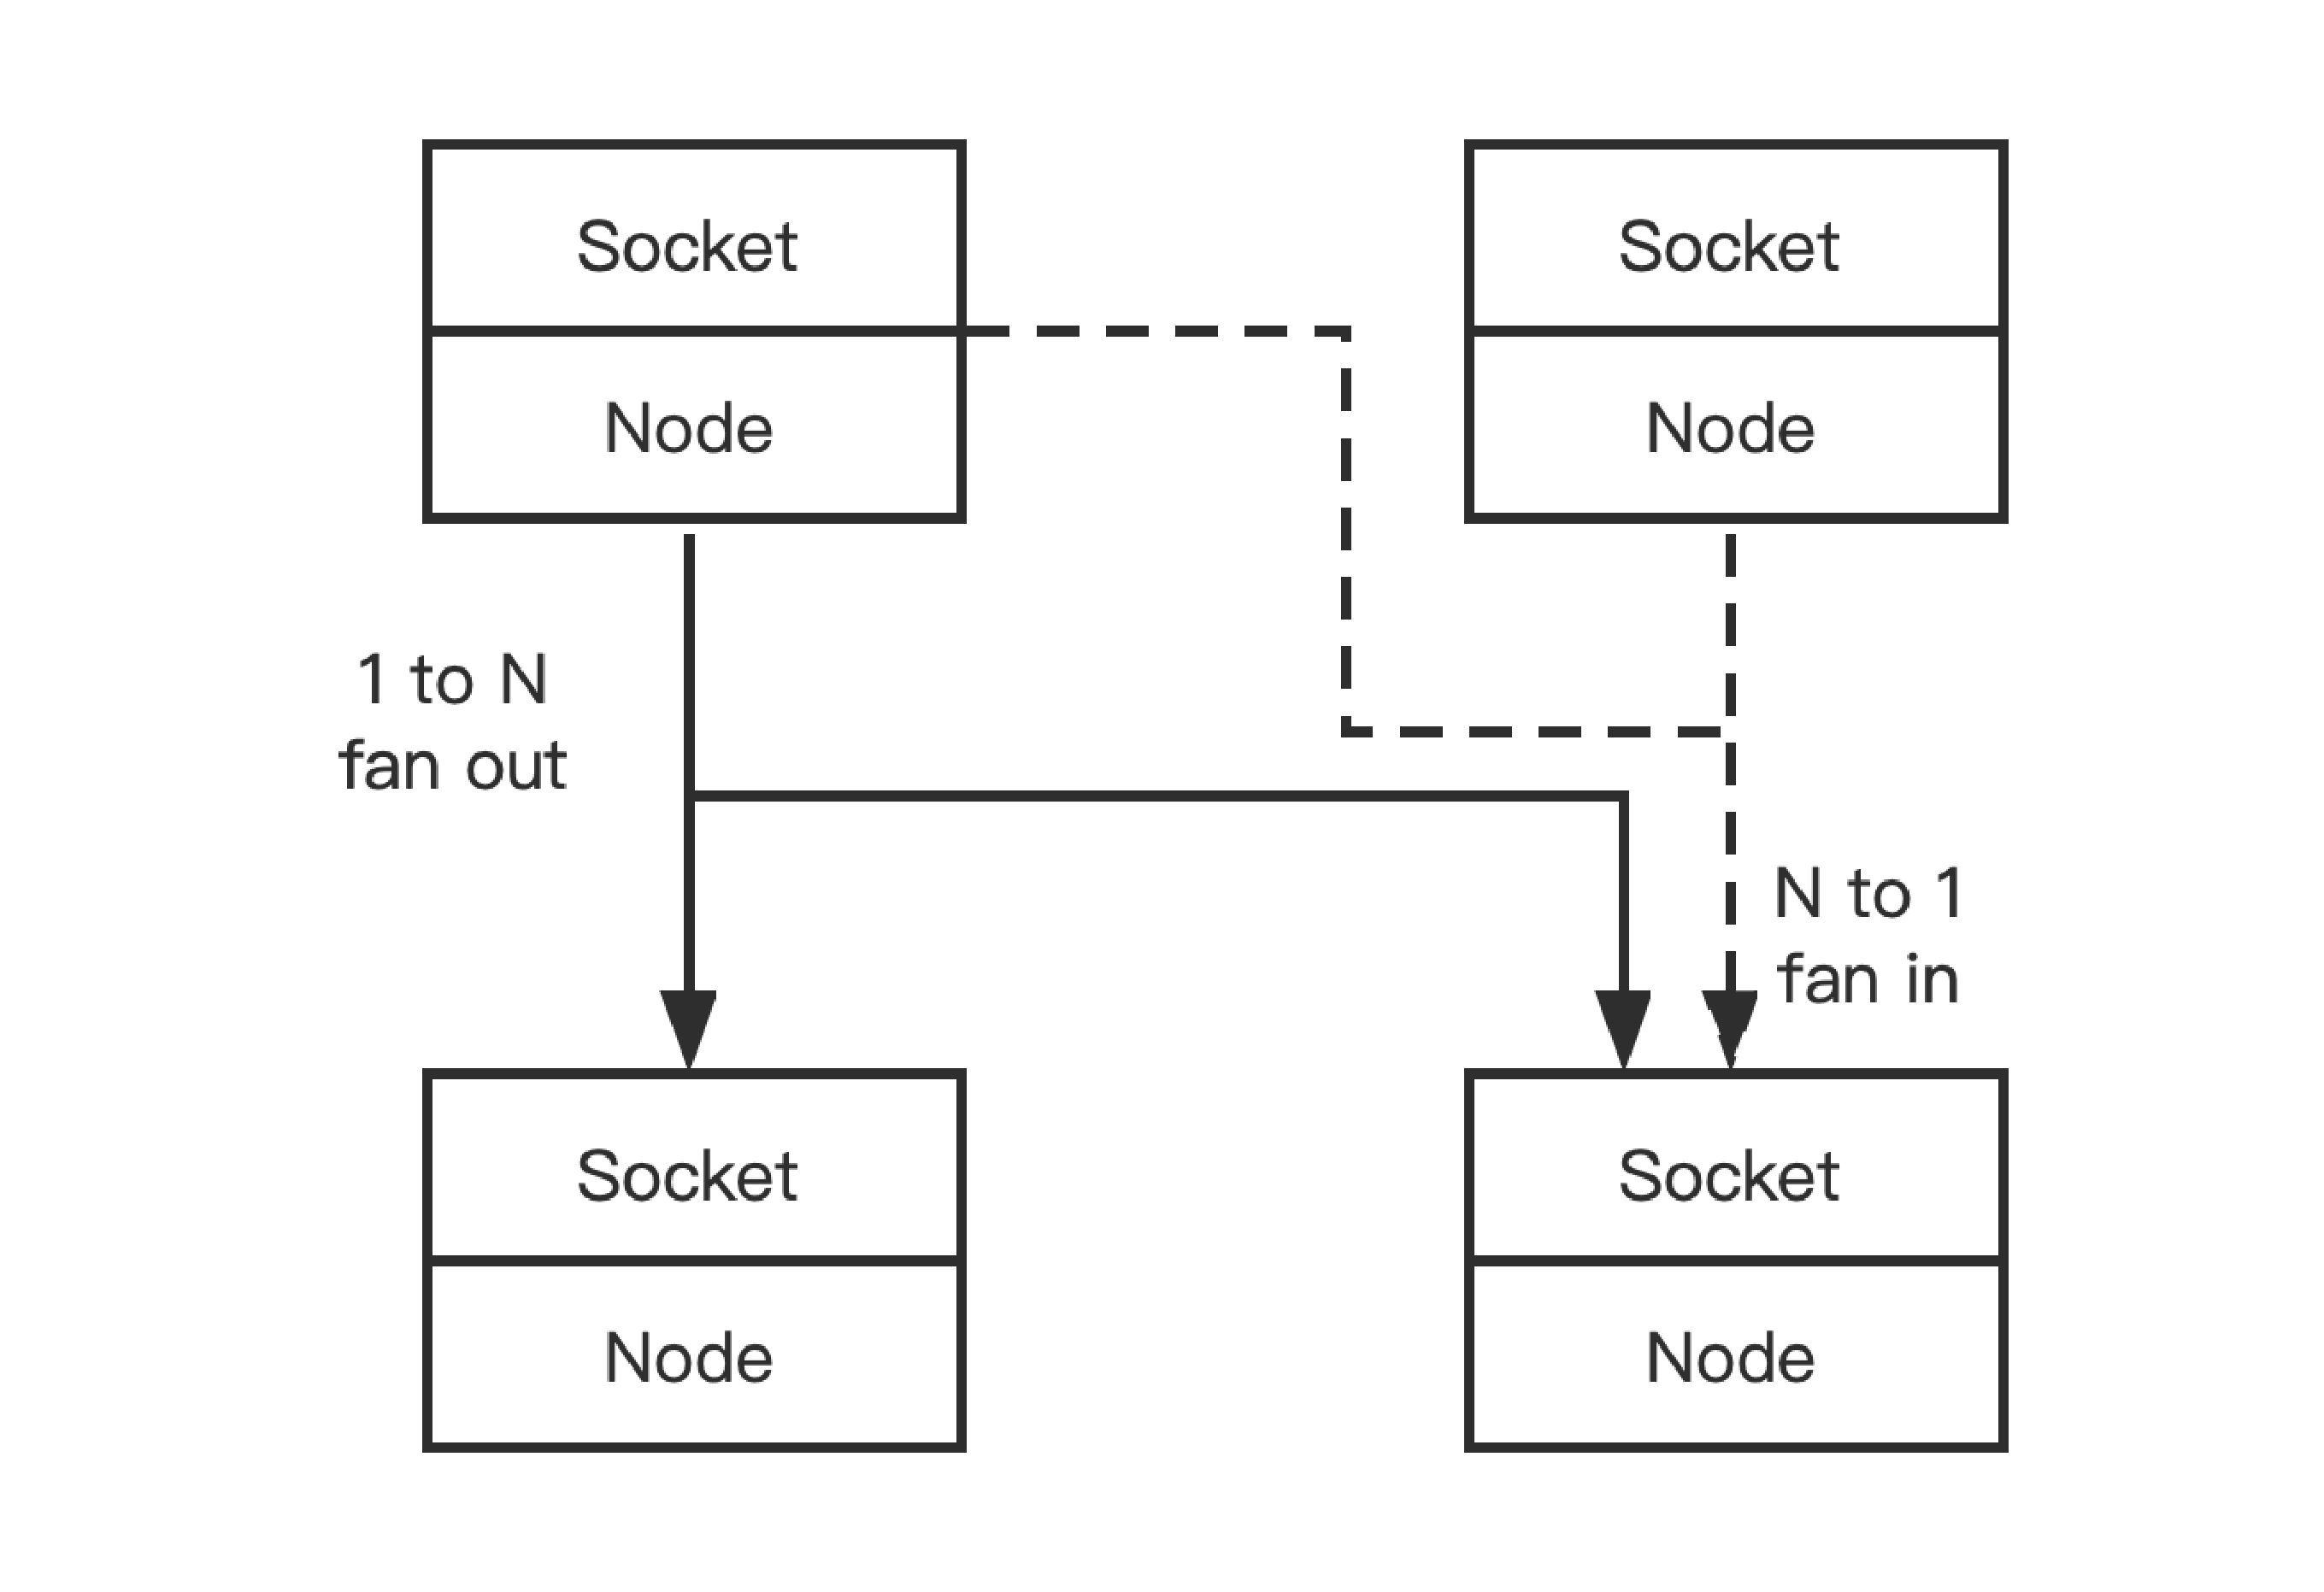
\includegraphics[width=0.65\textwidth]{fan-in-fan-out.pdf}
        \caption{ZeroMQ的扇入和扇出模型}
        \label{fan-in-fan-out}
      \end{figure}
\end{enumerate}

\subsection{ZeroMQ通信模式}
ZeroMQ共有四种通信模式:请求-应答模式、发布-订阅模式、管道模式和排他对接模式\cite{yyq},本节将对发布-订阅模式进行详细介绍。
% \subsubsection{请求-应答模式}
% 请求-应答模式将通信的双方角色划分为客户端和服务端,用于远程过程调用或任务分发。ZeroMQ提供了一共提供了
% 四种套接字实现此模式的需求:ZMQ\_REQ、ZMQ\_REP、ZMQ\_DEALER和ZMQ\_ROUTER。ZMQ\_REP和ZMQ\_REQ配对
% 使用时,必须相应请求必须有相应的应答方,否则请求发送后将一直阻塞至相应的应答方出现位置。同时,请求
% 和应答这两个动作必须有先后顺序,不能出现先应答后请求的情况\cite{wp}。图2.2展示了最简单的一对一的请求-应答模式的过程:
% \begin{figure}[H]
%     \centering
%     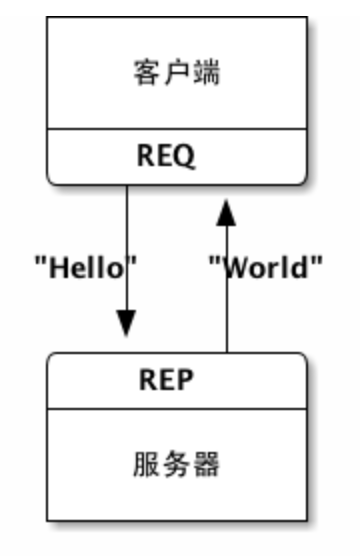
\includegraphics[width=0.28\textwidth]{2.2.png}
%     \caption{一对一的请求-应答模式过程}
%     \label{fig:5}
%   \end{figure}
% 客户端创建ZMQ\_REQ套接字后,填写请求的地址以及请求体的内容,发送后进入阻塞状态直到收到应答才
% 能解除阻塞重新调度队列进行后续的作业;服务端创建ZMQ\_REP套接字并持续监听某一个地址,当监听
% 到某个请求消息到来后对请求消息进行处理,处理完成后返回处理的结果给发出此请求的客户端。

% ZMQ\_REQ套接字和ZMQ\_REP套接字的连接关系既可以是一对一的,也可以是多对多的。当一个ZMQ\_REQ套接字
% 连接多个ZMQ\_REQ套接字时,ZeroMQ会将客户端的多个请求负载均衡到不同的服务端,如图2.3所示。当
% 多个ZMQ\_REQ套接字连接至一个ZMQ\_REP套接字时,服务端会公平地接收并处理不同的请求。
% \begin{figure}[H]
%     \centering
%     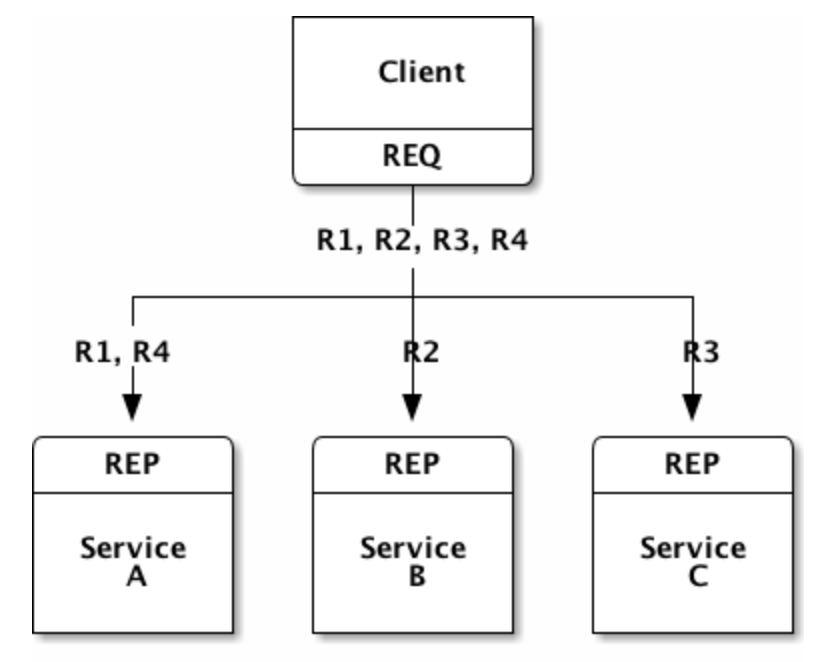
\includegraphics[width=0.6\textwidth]{2.3.png}
%     \caption{多请求负载均衡}
%     \label{fig:6}
%   \end{figure}
% 考虑到本文提出的自动驾驶运行时通信系统的各通信节点并不是固定不变的,节点之间的通信关系会随着时间动态地发生
% 变化,通信节点的绝对数量也会发生变化。通信系统中可能出现一个客户端请求多个服务端,也可能出现多个服务端
% 应答一个客户端。前一种情况下,添加一个新的客户端是容易实现的,只需要将负载均衡模块的服务端地址列表
% 告知新的客户端即可。但在后一种情况下,添加一个新的服务端是不容易实现的,需要将新的服务端地址通知到
% 每一个存在的客户端,并且这些客户端可能分布在不同的网络中,实现服务端与客户端的地址同步就会产生
% 大量的性能开销。

% 鉴于此类情况,ZeroMQ提供了ZMQ\_DEALER套接字和ZMQ\_ROUTER套接字来解决客户端服务端同步的问题。
% 用户可通过将多个ZMQ\_REQ套接字连接至ZMQ\_ROUTER套接字,所有的请求会通过公平排队转发给ZMQ\_DEALER
% 套接字,ZMQ\_DEALER套接字通过负载均衡的方式将所有请求发送给与其相连接的多个ZMQ\_REP套接字\cite{7360036}。
% ZeroMQ称这种方法为请求-应答代理,图2.4展示了使用代理的请求-应答模式的架构:
% \begin{figure}[H]
%   \centering
%   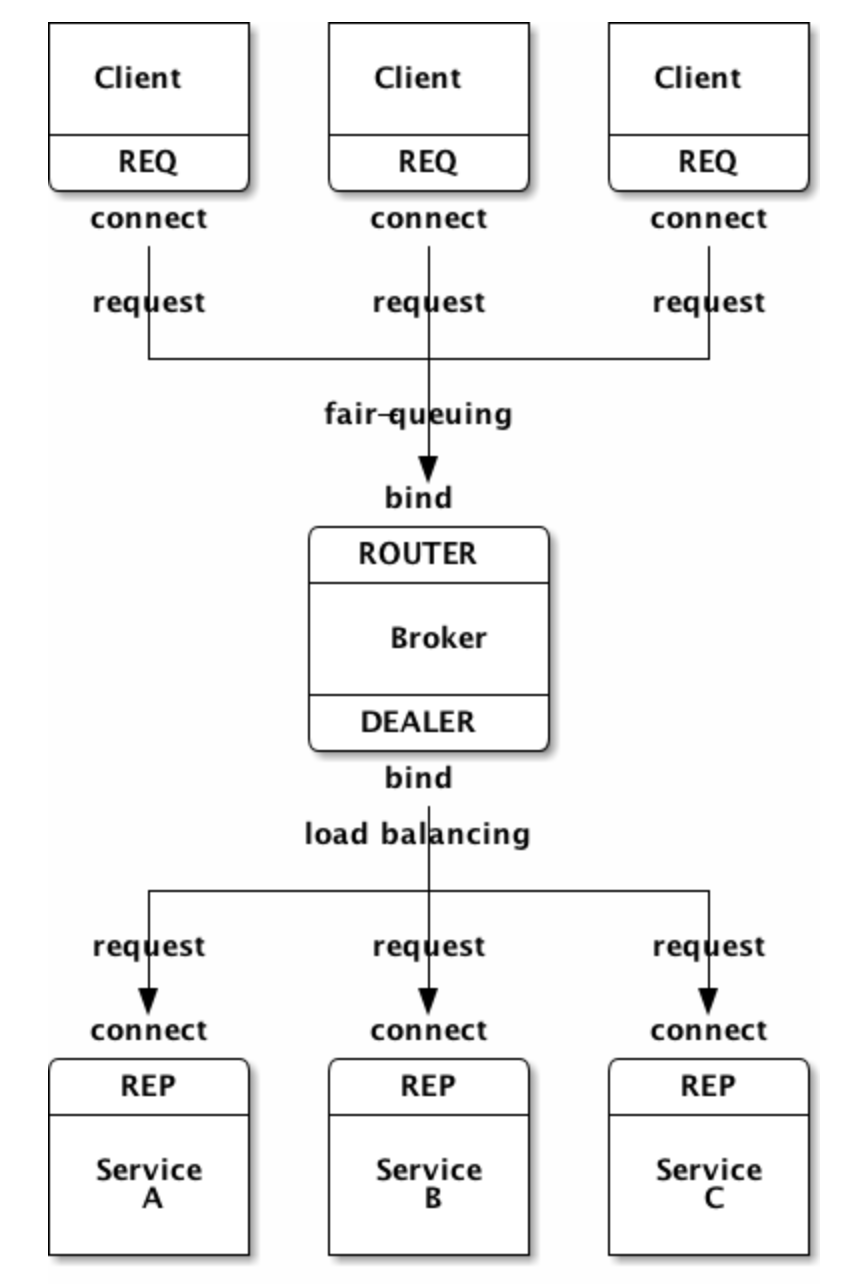
\includegraphics[width=0.5\textwidth]{2.4.png}
%   \caption{请求-应答代理架构}
%   \label{fig:7}
% \end{figure}
% 使用代理实现服务端与客户端动态变化的请求-应答模式的情况下,所有的客户端会在待发送的消息前插入空格后发送,
% ROUTER为了标识多个客户端发送的请求,会将收到的所有请求加上UUID(通用唯一识别码)对不同的客户端请求进行
% 区分,图2.5展示了使用代理后ZeroMQ数据帧的变化:
% \begin{figure}[H]
%   \centering
%   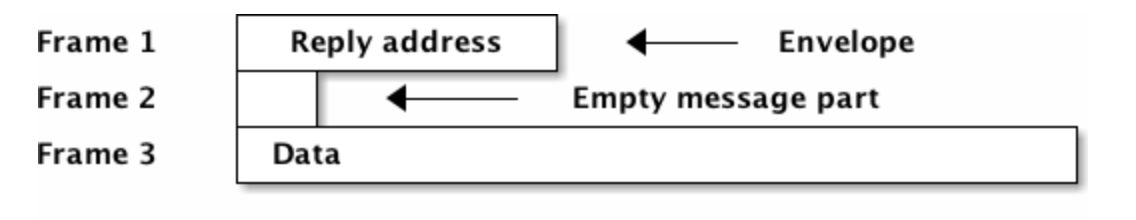
\includegraphics[width=1\textwidth]{2.5.png}
%   \caption{代理模式下的数据帧}
%   \label{fig:8}
% \end{figure}
% 其中帧3代表客户端实际的请求消息体,帧2是客户端发出请求前加上的空白消息,帧1是ROUTER在收到客户端请求
% 后加上的UUID。ROUTER收到请求消息并加上UUID后会交给DEALER通过负载均衡发送到不同的服务端进行处理。
% 服务端收到经过处理的请求消息后会直接取出帧3处理实际的请求体,处理完成后会将帧3替换为处理后的响应消息返回
% 给DEALER,最后ROUTER会检验数据帧,如果数据帧缺少UUID则直接丢弃本数据帧,检验无误后根据UUID将
% 响应消息返回给与UUID关联的客户端。
% \subsubsection{发布-订阅模式}
发布-订阅模式将通信的双方角色划分为发布者与订阅者。ZeroMQ提供了四种套接字实现该模式的相关需求:
ZMQ\_SUB、ZMQ\_PUB、ZMQ\_XSUB和ZMQ\_XPUB。ZMQ\_SUB与ZMQ\_XSUB套接字作为订阅者,ZMQ\_SUB套接字只能
订阅消息,ZMQ\_XSUB套接字既可以订阅消息也可以发布消息。ZMQ\_PUB与
ZMQ\_XPUB作为发布者,ZMQ\_PUB套接字只能发布消息,ZMQ\_XPUB套接字既可以发布消息也可以订阅消息。
发布者套接字与订阅者套接字之间的连接关系可以是一对一的,也可以是多对多的。图\ref{1-N-pub-sub}是一个发布者连接多个订阅者的模式。
\begin{figure}[H]
  \centering
  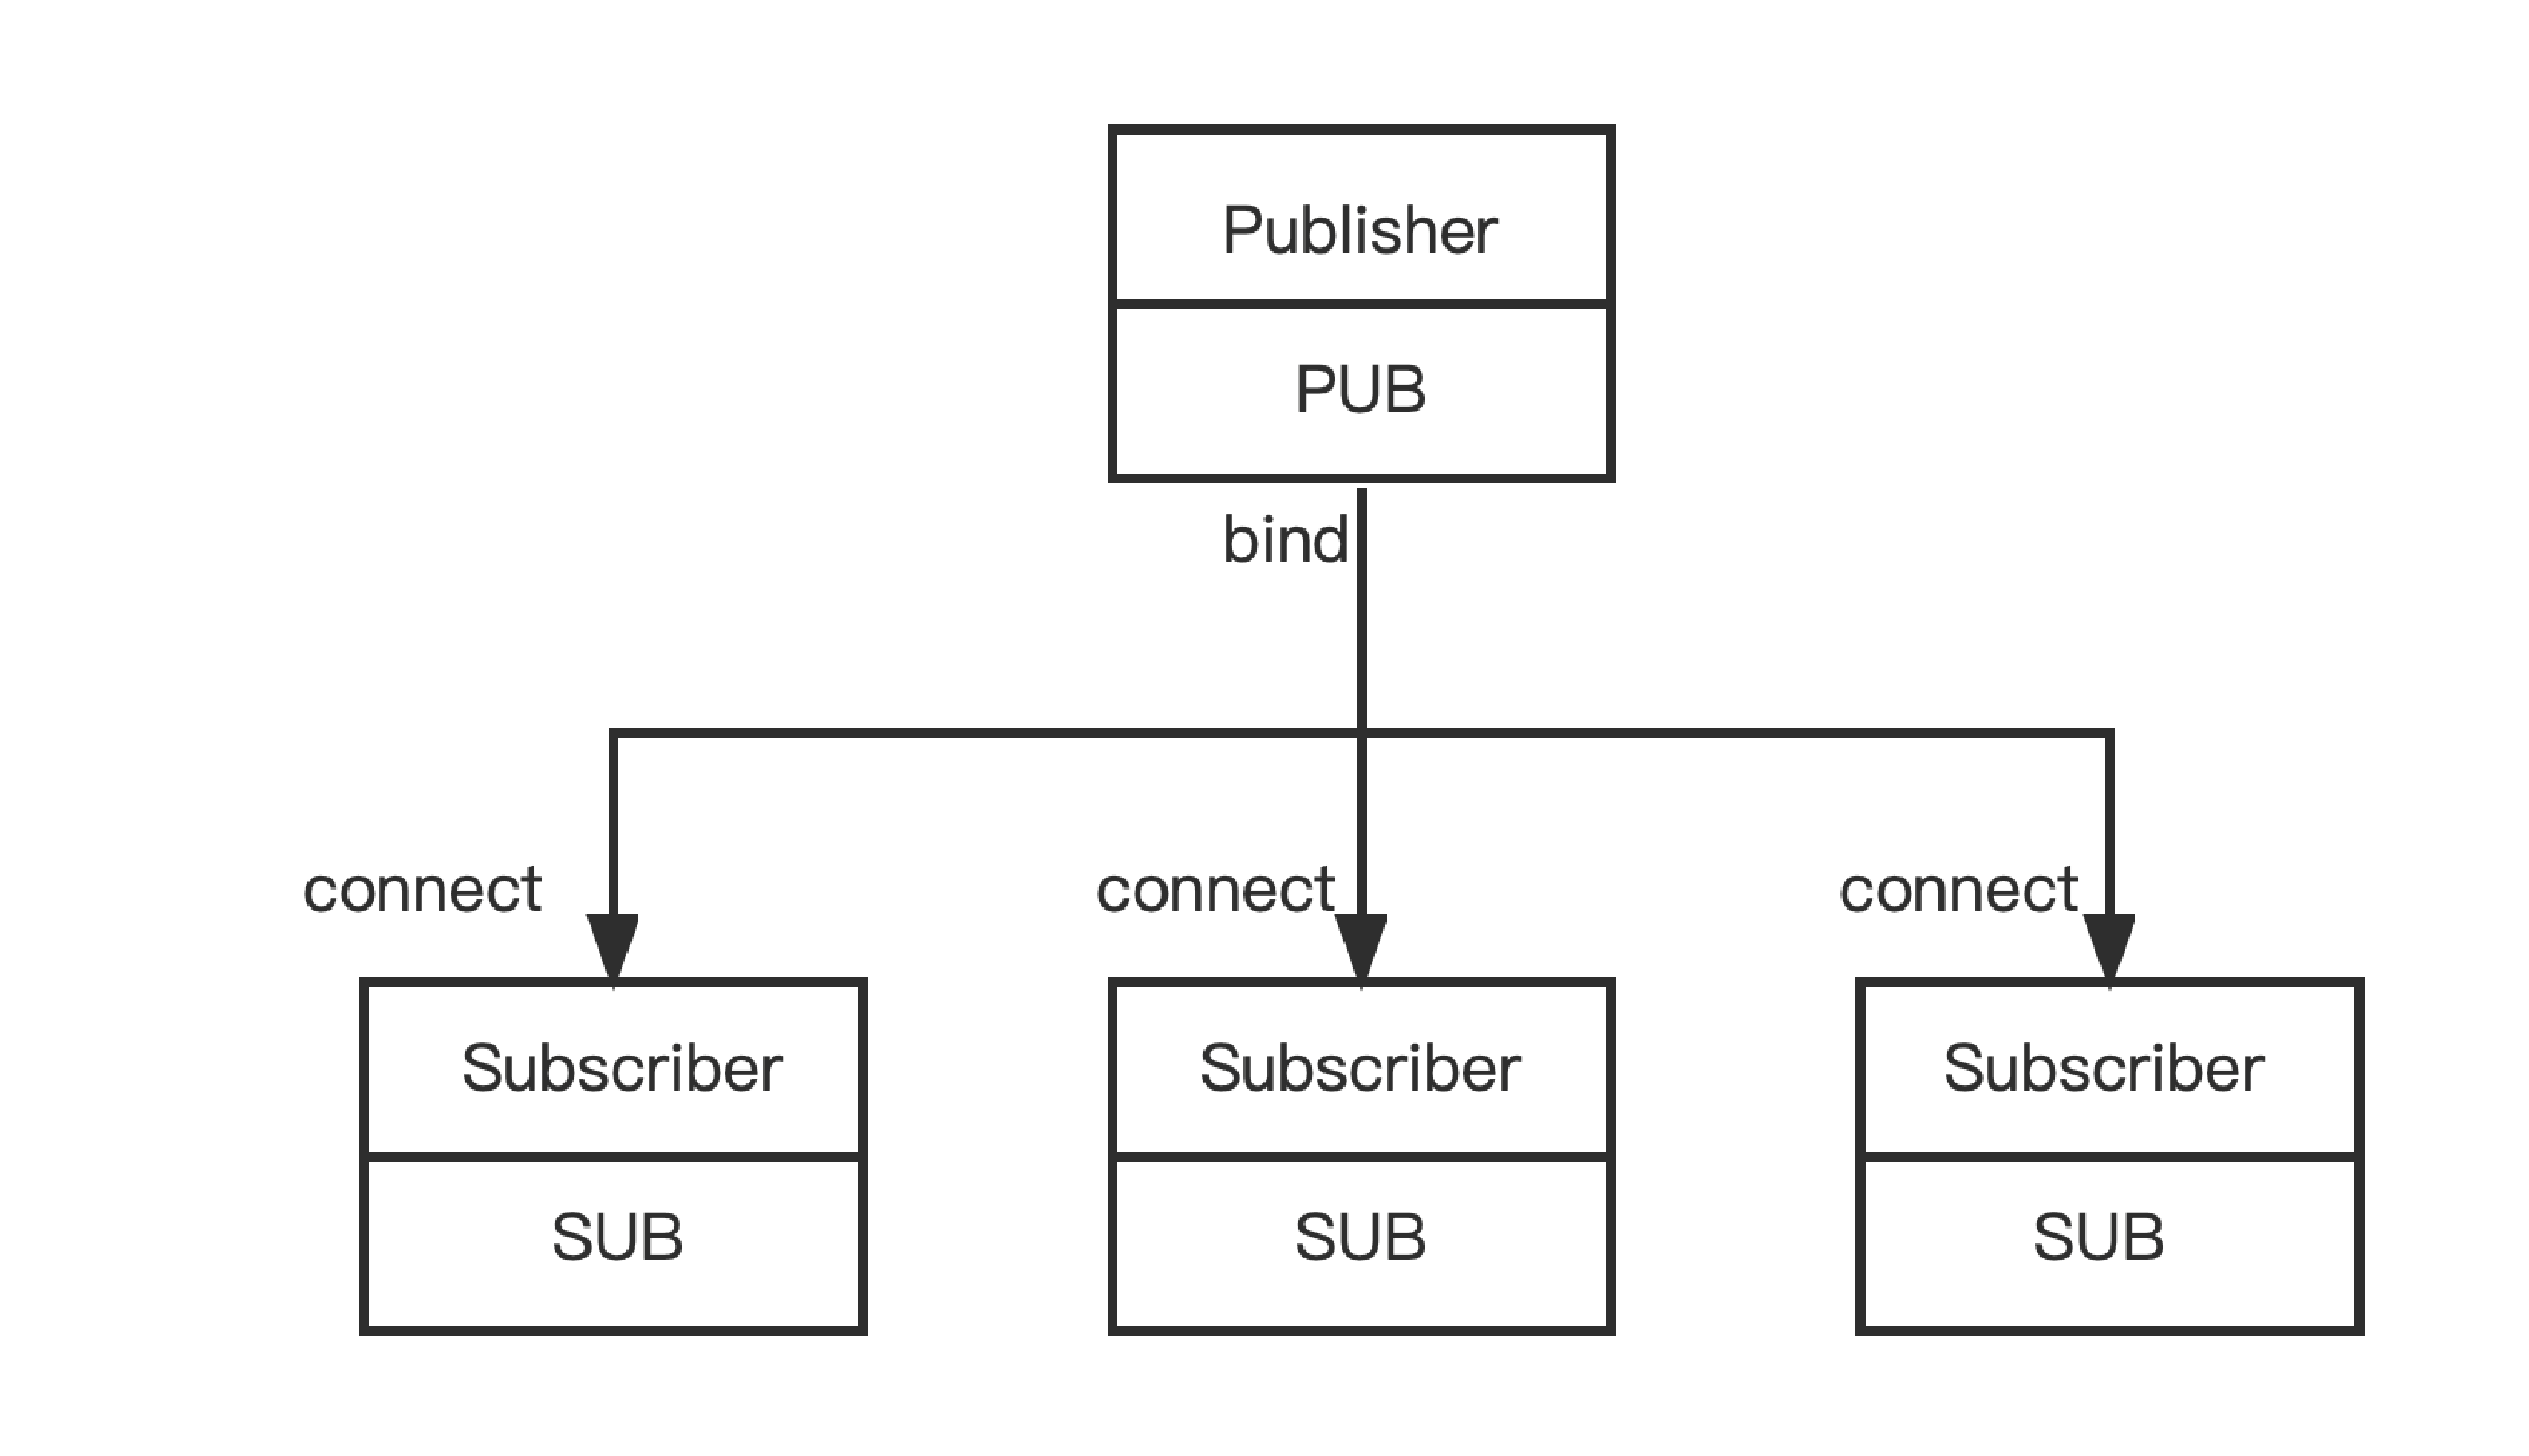
\includegraphics[width=0.7\textwidth]{1-N-pub-sub.pdf}
  \caption{一对多发布-订阅模式}
  \label{1-N-pub-sub}
\end{figure}

使用发布-订阅通信模式会面临发布者与订阅者动态变化的问题,开发者通过
使用ZMQ\_XSUB与ZMQ\_XPUB套接字实现发布-订阅代理,这两个套接字既可以发送消息也可以接收消息,基于这两种套接字
开发者可以开发出发布者与订阅者之间的通信代理装置。
图\ref{N-N-pub-sub}展示了使用代理解决发布者与订阅者动态变化问题的方法。
所有的发布者与订阅者不直接连接而是连接到代理装置,代理装置通过ZMQ\_XSUB获取所有发布者发布的消息,随后通过代理装置将这些
消息转通过ZMQ\_XPUB发布至所有订阅者,从而实现消息的间接发布。代理装置变动的频率相较于发布者与订阅者较低,代理装置可以灵活应对分布式
通信系统等使用场景中频繁新增或减少的发布者与订阅者。
\begin{figure}[H]
  \centering
  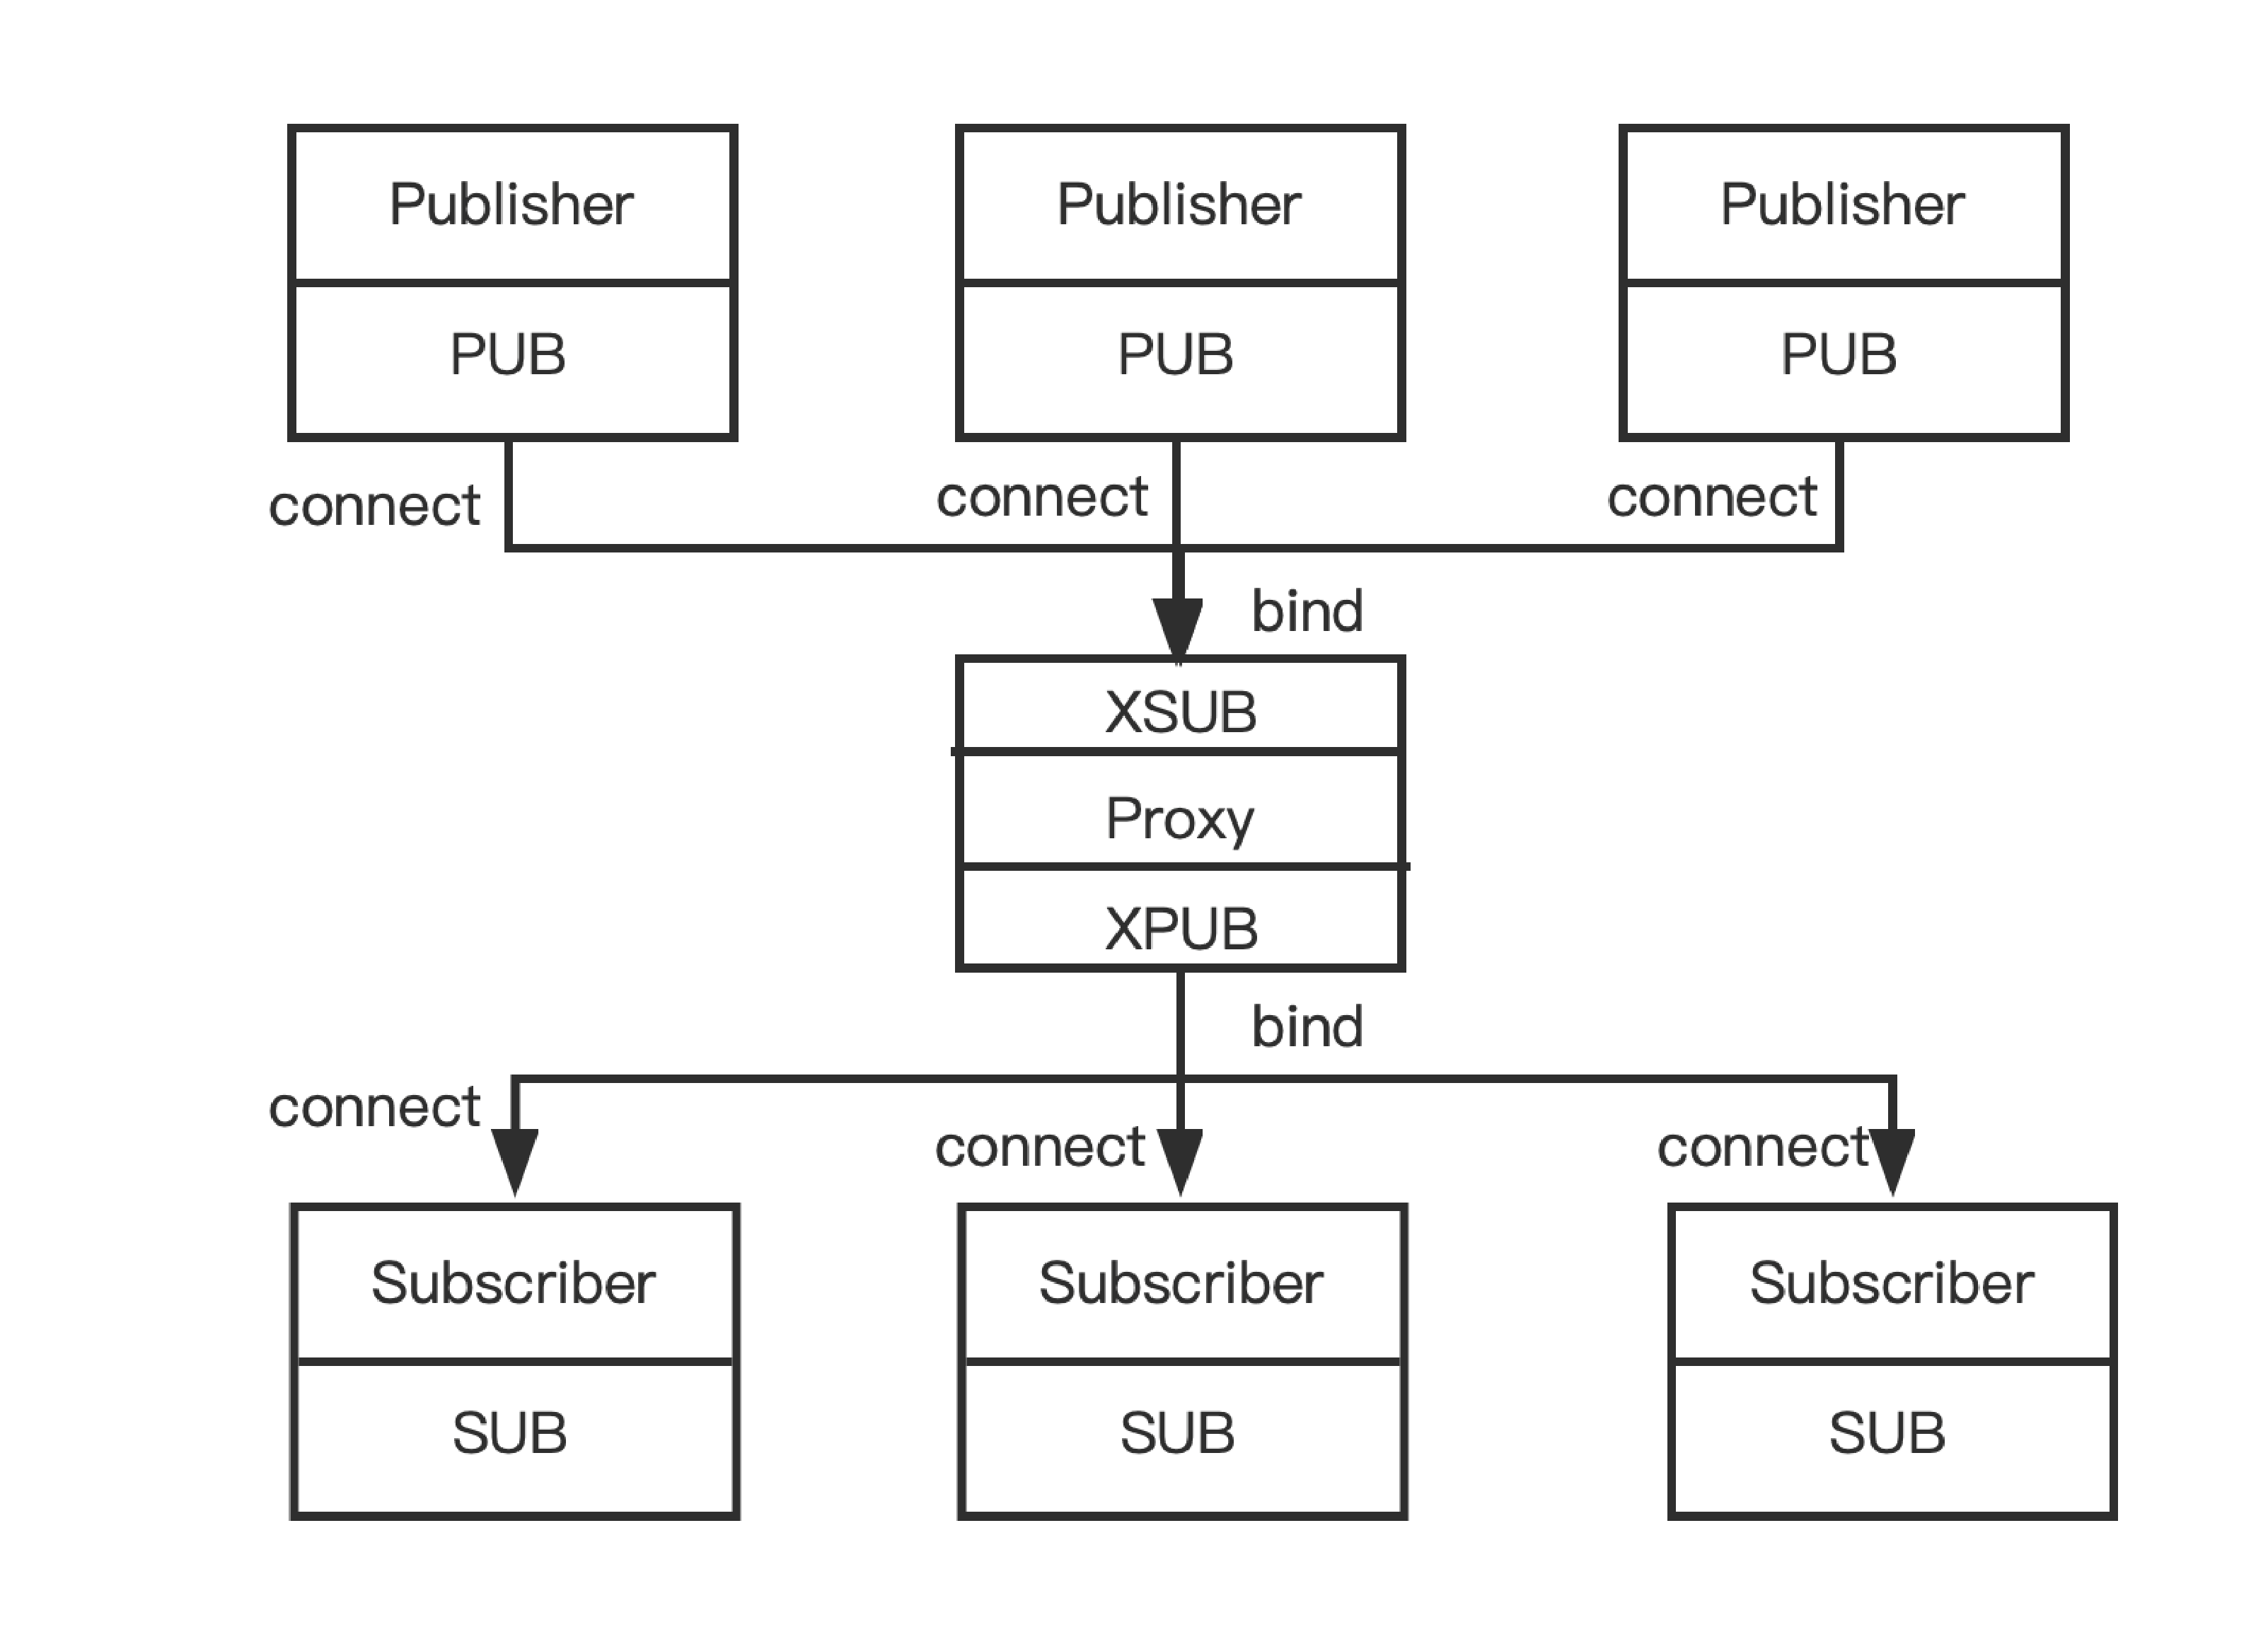
\includegraphics[width=0.7\textwidth]{N-N-pub-sub.pdf}
  \caption{发布-订阅代理架构}
  \label{N-N-pub-sub}
\end{figure}

开发中使用ZeroMQ的发布-订阅通信模式进行通信时,需要使用zmq\_socketopt函数设置ZMQ\_SUB套接字设置为ZMQ\_SUBSCRIBE属性,
如果不设置将无法订阅到任何消息。该函数的作用是为ZMQ\_SUB套接字设置需要过滤的消息,设置后ZMQ\_SUB套接字会将
所有符合过滤条件的消息丢弃。在ZeroMQ 2.1.0 stable release版本中消息过滤功能由订阅端完成,发布者并不会
根据每个订阅者的过滤条件选择性地发布消息,而是发布所有消息。

\subsection{ZeroMQ传输协议}
ZeroMQ提供了三种单播传输协议(tcp, ipc, inproc)和两种广播传输协议(epgm, pgm)。本系统没有使用广播传输协议,故本节只对
三种单播传输协议进行介绍。

ZeroMQ中的tcp传输协议基于计算机网络中传输层中的TCP进行二次封装,在TCP报文中的数据部分加入了ZeroMQ消息的
消息大小及消息体。该传输协议地址在ZeroMQ中以tcp://ip\_address:port(如tcp://localhost:8888)的形式出现,
当开发者将ZMQ\_PUB和ZMQ\_SUB套接字连接至以tcp为开头的通信地址时,ZeroMQ将会自动选择TCP网络通信的方式
进行通信。使用tcp传输协议传输消息时消息将会经过操作系统的网络协议栈,打包拆包等操作存在一定的通信性能开销,但对不同操作系统
的兼容性较好。

与ZeroMQ的tcp传输协议相类似的是ipc传输协议,传输协议地址在ZeroMQ中以ipc://any\_address(如ipc://test)的形式出现。该协议使用Unix domain socket(Unix域socket)作为进程间通信
的手段,为处于同一台物理机的发布者与订阅者提供通信。Unix domain socket是POSIX操作系统的一个标准,
目前ZeroMQ尚未支持Windows系统使用该传输协议,只支持在遵循POSIX标准的操作系统中使用,
因此该传输协议对操作系统的兼容性不如tcp传输协议。
但ipc传输协议并不需要经过操作系统的网络协议栈,免去了打包拆包等操作带来的通信开销,通信效率优于tcp传输协议。

此外,ZeroMQ还提供了inproc传输协议用于同一台物理机同一个进程中的发布者与订阅者通信,传输协议地址在ZeroMQ中以inproc://any\_address(如inproc://test)
的形式出现。该传输协议使用消息的指针将发布者的消息传递给订阅者,该传输协议是三种单播传输协议中效率最高。

\subsection{ZeroMQ性能表现}
国外文章\cite{mqcompare}比较了MSMQ、ActiveMQ、RabbitMQ和ZeroMQ每秒钟可以发送和接受的消息数量,
从表\ref{messge_queue_compare}可以看出ZeroMQ拥有比较明显的优势。
\begin{table}[htb]
  \centering\small
  \caption{常见消息队列每秒收发消息数量对比\cite{mqcompare}}
  \label{messge_queue_compare}
  \begin{tabular}{ccccc}
    \toprule
    & ZeroMQ & RabbitMQ & ActiveMQ & MSMQ \\
    \midrule
    接收 & 88699 & 12281 & 6453 & 7021 \\
    发送 & 242659 & 12278 & 6452 & 11406 \\
    \bottomrule
  \end{tabular}
\end{table}

通过本节对ZeroMQ的介绍,可以得出ZeroMQ使用起来非常方便,并且其内部实现的代理可以灵活
应对分布式通信系统动态变化的通信节点,同时其性能也较其他同类产品有比较明显的优势,最终本文统选用
ZeroMQ作为网络通信的工具。

\section{序列化技术}
序列化技术(也称列集技术)包括序列化和反序列化两部分,序列化是将某一种格式(如C++结构体、Java对象等)进行一系列
的处理并最终生成二进制序列的过程,反序列化则是序列化的相反过程\cite{zj,wangbinbin}。本文使用序列化技术主要有以下几点
理由:
\begin{enumerate}
  \item 本文研究的通信系统是具备分布式通信能力的,这代表不同网络中的通信节点需要使用网络通信来传输相关的信息。
  而基于TCP/IP的网络通信不支持直接传输某个编程语言中的类或结构体,必须要将相关数据类型序列化成
  二进制序列才可以在网络中进行传输。
  \item 序列化技术可以将某种语言的数据类型转换成与语言和平台无关的二进制序列,这个功能代表了
  使用序列化来进行数据的传输可以跨平台跨语言。只要在序列化技术支持的平台和语言列表中进行开发就不需要
  为不同平台和语言进行额外的适配工作,大大简化了开发工作量。
  \item 序列化技术可以大大减少原数据的大小。从网络通信方面来看,减少通信需要的带宽并加快了数据传输的速度。
  从基于共享内存的进程间通信来看,减少了需要向系统申请的共享内存空间。这种优势在传输小数据时不是很明显,
  但在自动驾驶中摄像机的图像数据大小会达到MB级别,在这种情况下序列化对原始数据的压缩就显得尤为重要。
\end{enumerate}
本文选用Google开源的Protocol Buffer作为序列化工具。Protocol Buffer是一种高性能、易于使用且
扩展性较强的数据存储格式,支持Python、C++和Java语言\cite{sxy}。

使用Protocol Buffer最重要的一步就是编写IDL(交互式数据语言)文件,通常IDL的编写是依据使用者
已有的数据类型进行对照进行的,即参照已有的C+结构体或Java对象的内部数据成员进行编写。图\ref{IDL_compare}展示
了如何根据C++结构体编写IDL。
\begin{figure}[H]
  \centering
  \subfigure[结构体]{
    \label{IDL_compare_1}
    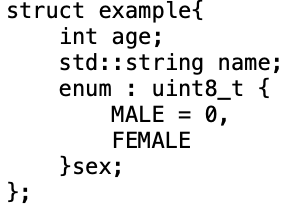
\includegraphics[width=0.4\textwidth]{2.8-0.png}}
  \subfigure[IDL]{
    \label{IDL_compare_2}
    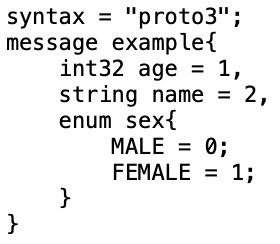
\includegraphics[width=0.38\textwidth]{2.8-1.png}}
  \caption{根据C++结构体编写对应IDL}
  \label{IDL_compare}
\end{figure}
通过比较图\ref{IDL_compare_1}与图\ref{IDL_compare_2}可以看出,IDL的编写基本和C++等主流语言保持了一致规则,学习IDL编写的
成本并不大。IDL提供了一系列的关键字供使用者实现更为复杂的序列化规则,不止包括定义一个数据类型,
还可以定义服务的接口等高级功能,本文就不再赘述了。Protocol Buffer中的IDL是向后兼容的,当根据业务需求修改
IDL时并不会发生大规模重构反序列化代码以及IDL的md5值不一致的情况。而ROS中的IDL(.msg和.srv文件)没有
向后兼容的特性,当IDL发生改变后必须重构代码,否则会出现md5值不一致导致无法完成通信的情况。

常见的序列化技术并不只有Protocol Buffer一种,XML和JSON也是应用非常广泛的序列化技术方案,但本文
选用Protocol Buffer而不使用其他序列化技术主要有性能上和序列化技术本身的数据表达能力的考虑。
表\ref{serialize_tool_compare}展示了Protocol Buffer、XML以及JSON表达相同一个数据类型的格式。
\begin{table}[H]
  \centering\small
  \caption{三种序列化技术描述数据的格式对比\cite{6215346}}
  \label{serialize_tool_compare}
  \begin{tabular}{cc}
    \toprule
    序列化技术   &  格式                                       \\
    \midrule
    Protocol Buffer & message example\{int32 age = 1;string name = 2;\}  \\
    JSON & \{"age" : 1, "name" : "example"\}   \\
    XML & <example><age>1</age><name>example</name></example>       \\
    \bottomrule
  \end{tabular}
\end{table}
从表中可以看出Protocol Buffer相较于其他两种序列化方案,它对描述一个数据类型的描述格式非常
直观,每一个成员变量的类型在编写IDL时就直接确定。而XML和JSON对一个数据类型描述的格式并不能
让使用者直观地看出每一个变量的具体类型,且当数据类型本身非常复杂时他们的描述格式阅读起来更为困难。

Protocol Buffer在性能方面也较XML和JSON有明显的优势。表\ref{serialize_performance_compare}列出了这三种
序列化方案序列化同一份数据的耗时、反序列化同一份数据的耗时以及序列化后的字节大小\cite{proto}:
\begin{table}[H]
  \centering\small
  \caption{三种序列化技术性能对比}
  \label{serialize_performance_compare}
  \begin{tabular}{cccc}
    \toprule
    序列化技术 & 序列化耗时(ms) & 序列化后字节数(Byte) & 反序列化耗时(ms)                                       \\
    \midrule
    Protocol Buffer & 241 & 117 & 190 \\
    JSON & 871 & 255 & 786 \\
    XML & 1383 & 474 & 1781 \\
    \bottomrule
  \end{tabular}
\end{table}


本小节阐述了为什么在本文的自动驾驶运行时通信系统中需要使用序列化技术,
通过对比Protocol Buffer、XML以及JSON描述数据类型格式的可阅读性,以及列出实际数据对比了
三种序列化技术的性能参数,最终本文选用Protocol Buffer作为序列化工具。
\section{远程服务调用}
远程服务调用(Remote Proceduce Calls, RPC)是由Nelson于1982年提出的一种跨进程消息同步的一种通信机制\cite{Andrew}。
RPC屏蔽了底层的通信细节和传输错误并为分布式系统提供了灵活便捷的通信功能。
RPC的具体实现包括RPC-JSON和RPC-XML\cite{2011TOWARD,2013Web},此外还有许多不同类型的实现,但RPC的通信方法是类似的,不同的实现方法
仅在传输的数据格式本身有差异。

RPC解决的问题是实现分布式系统中各个通信单元调用不同服务的过程
像本地调用一样方便。RPC为了保证调用远程的服务的透明性,也引入了代理的概念\cite{5694349}。图\ref{rpc_flowchart}是一次RPC调用的流程图。
\begin{figure}[H]
  \centering
  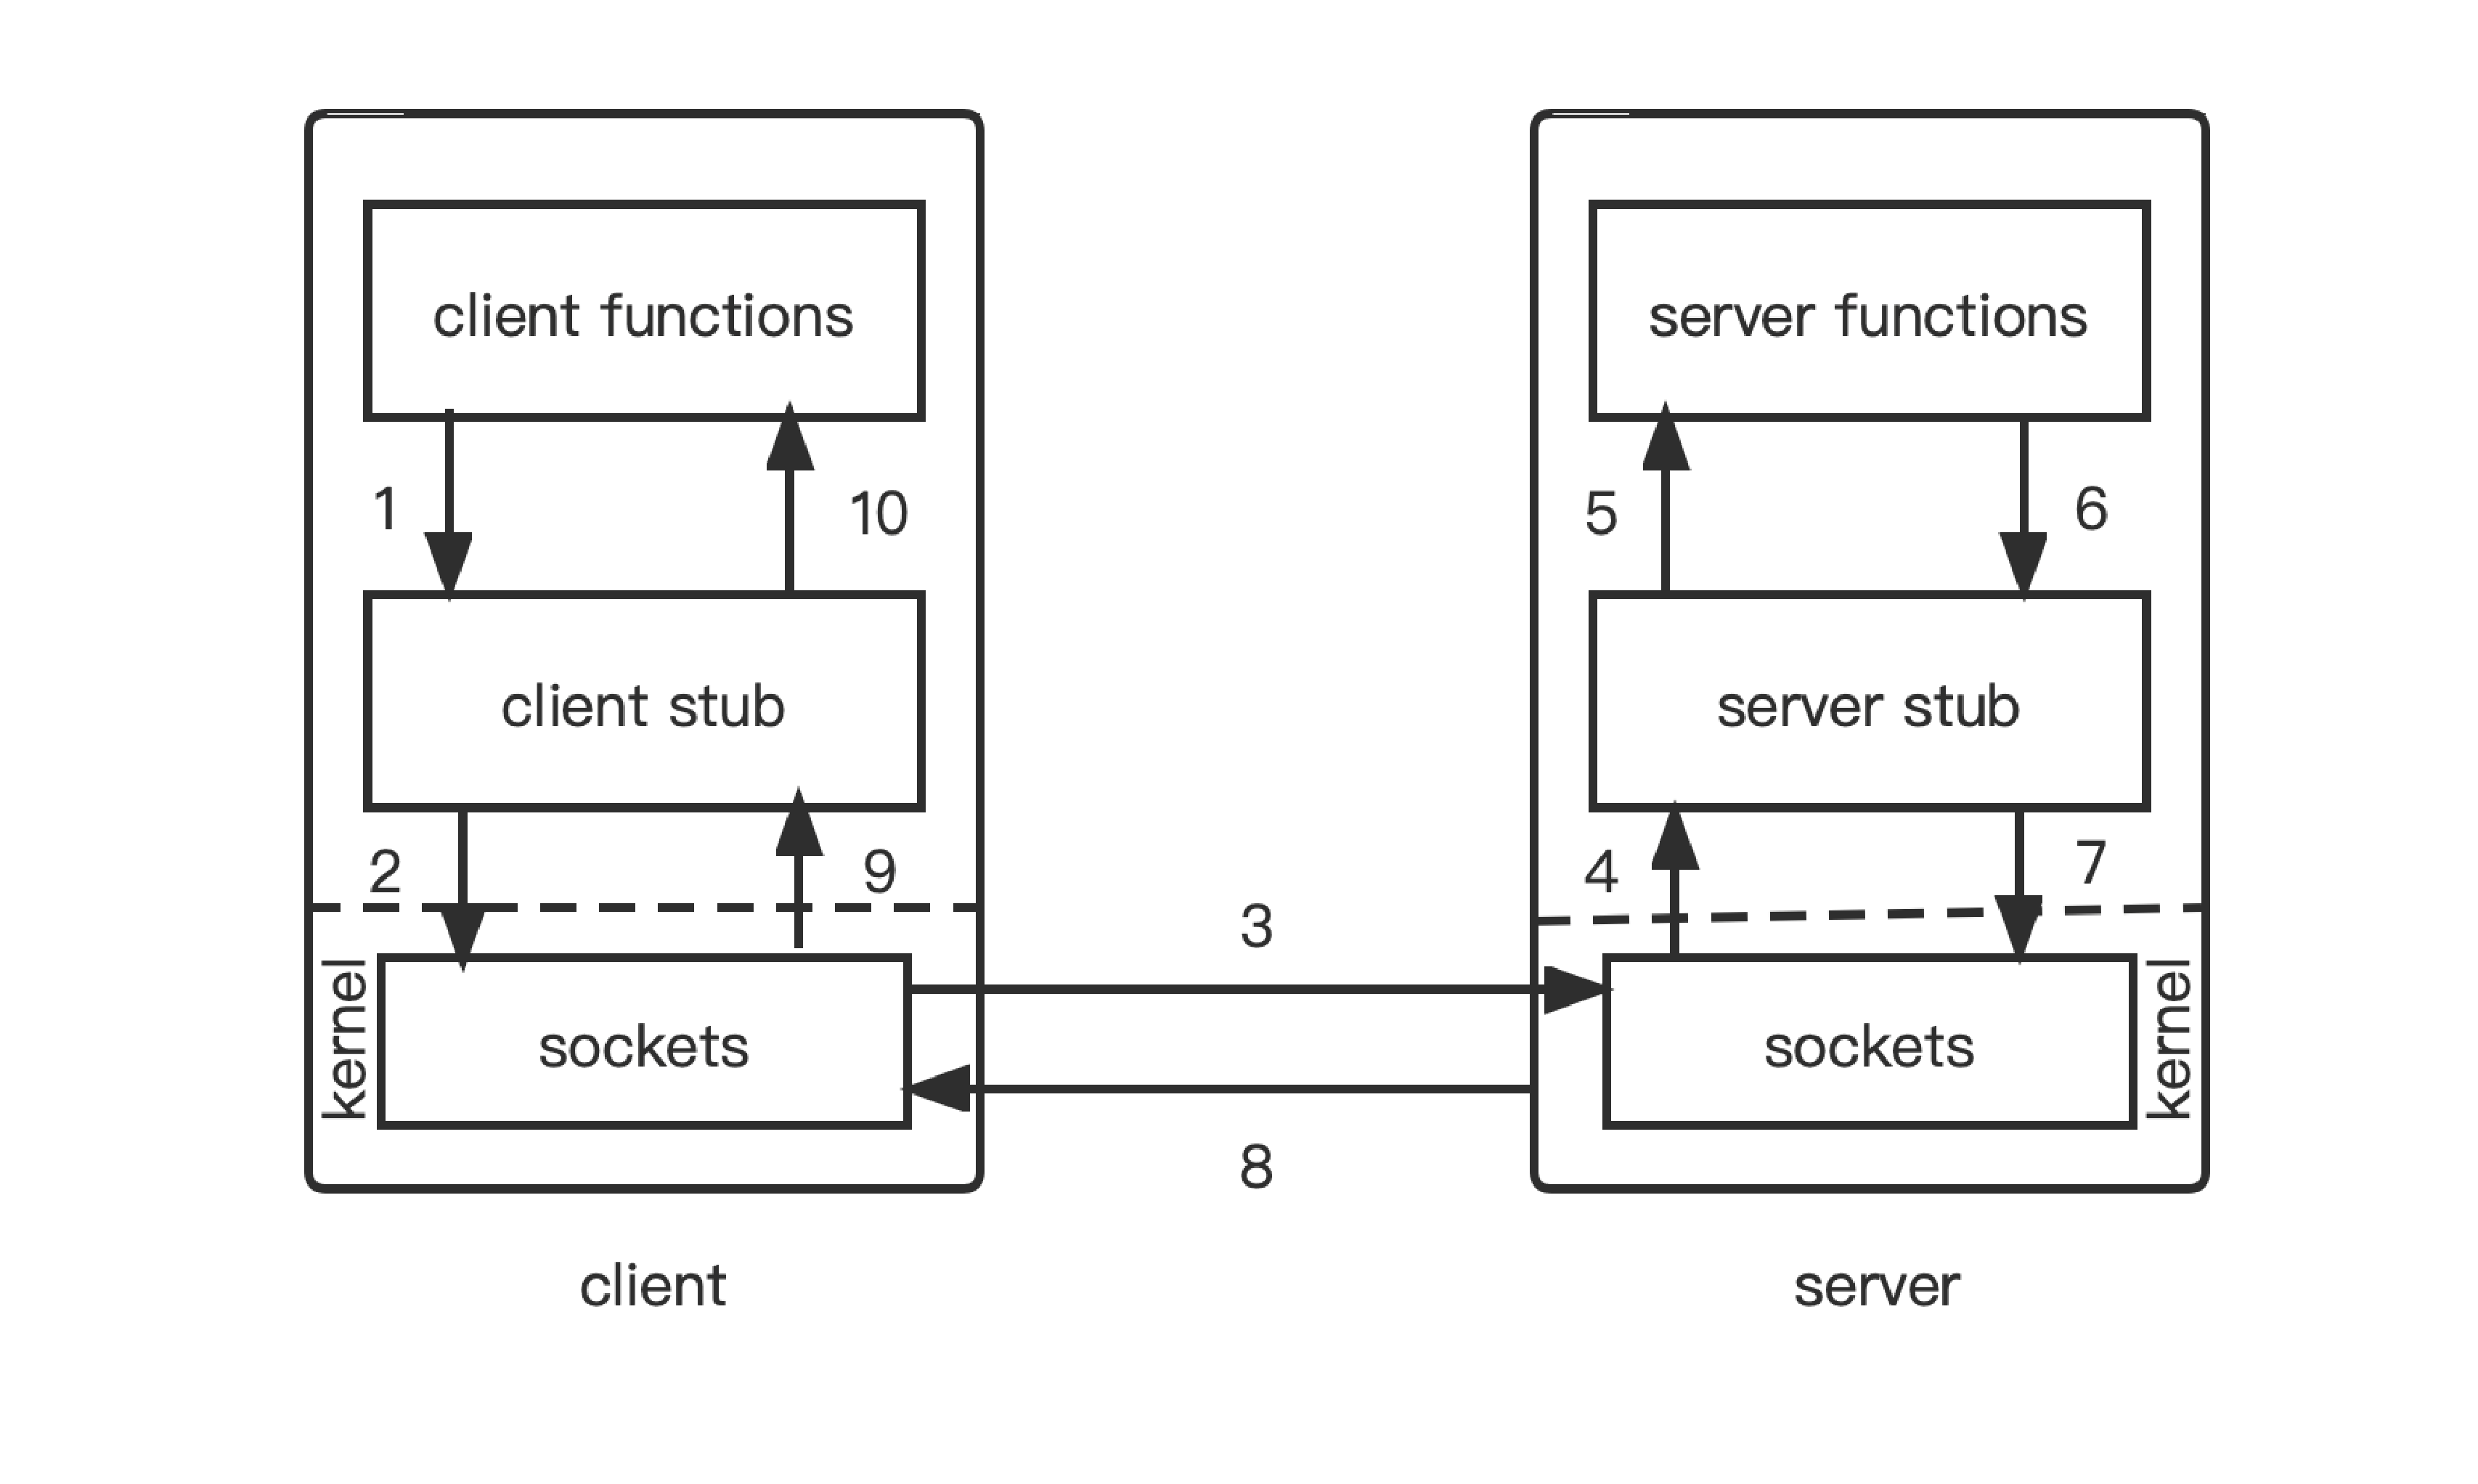
\includegraphics[width=0.8\textwidth]{rpc_flowchart.pdf}
  \caption{RPC调用流程}
  \label{rpc_flowchart}
\end{figure}
从图\ref{rpc_flowchart}可以看出,RPC调用过程主要分为以下几个步骤:
\begin{enumerate}
  \item 客户端发起调用之前,首先要确定需要调用什么服务。服务端为了将自身提供的不同服务做区分,会将
  每一个提供的服务加上标识(Call ID),以此让客户端能够指定调用某一个服务。客户端确定调用的服务后,
  需要将参数一并发送给本地的RPC代理。在上一节提到过,网络传输的内容只能是二进制的序列,所以客户端
  如果需要传输字符串之外的参数必须要将参数序列化为二进制序列。
  \item 客户端的RPC代理收到Call ID以及相关参数后,找到提供此服务的服务端并将调用信息以网络的形式
  传输给服务端。
  \item 服务端的RPC代理收到服务调用请求后,首先会对调用信息反序列化取得Call ID以及参数,根据
  Call ID找到本地对应的服务结合参数进行处理,处理完成后将结果序列化并通过RPC代理返回客户端代理。
  \item 客户端通过代理取得本次服务调用的结果,反序列化完成后就可以继续之后的作业。
\end{enumerate}

RPC解决的问题契合了本文提出系统的关键问题,即如何保证分布式通信系统在动态场景下所有通信节点都有方法
获取最新的网络拓扑。本文基于RPC的思想以及实际提供的技术方案并且融合了注册中心的概念,在主节点中
向通信节点提供服务调用,包括查询网络拓扑以及根据新增节点发送的RPC请求向所有有关的节点发送网络拓扑信息。

\section{共享内存}
共享内存是操作系统提供的进程间通信方式之一,也是最重要的一种进程间通信方式,其通信效率相较于其他通信方式
有明显的优势。共享内存的原理是将两个或多个独立的进程的一段虚拟地址映射到同一块物理地址,这些进程共同使用
物理地址的某一个区域。进程对共享内存的修改直接作用在物理内存上,不会发生用户态与内核态之间的数据拷贝,所以
共享内存并没有多余的数据拷贝,称零拷贝(零拷贝并不代表一次数据拷贝都没有发生,零的概念是相对于拷贝次数更多的通信方式而言)。
图\ref{IPC_compare}对比了共享内存与TCP socket读写数据过程的对比。
\begin{figure}[H]
  \centering
  \subfigure[共享内存]{
    \label{IPC_compare_1}
    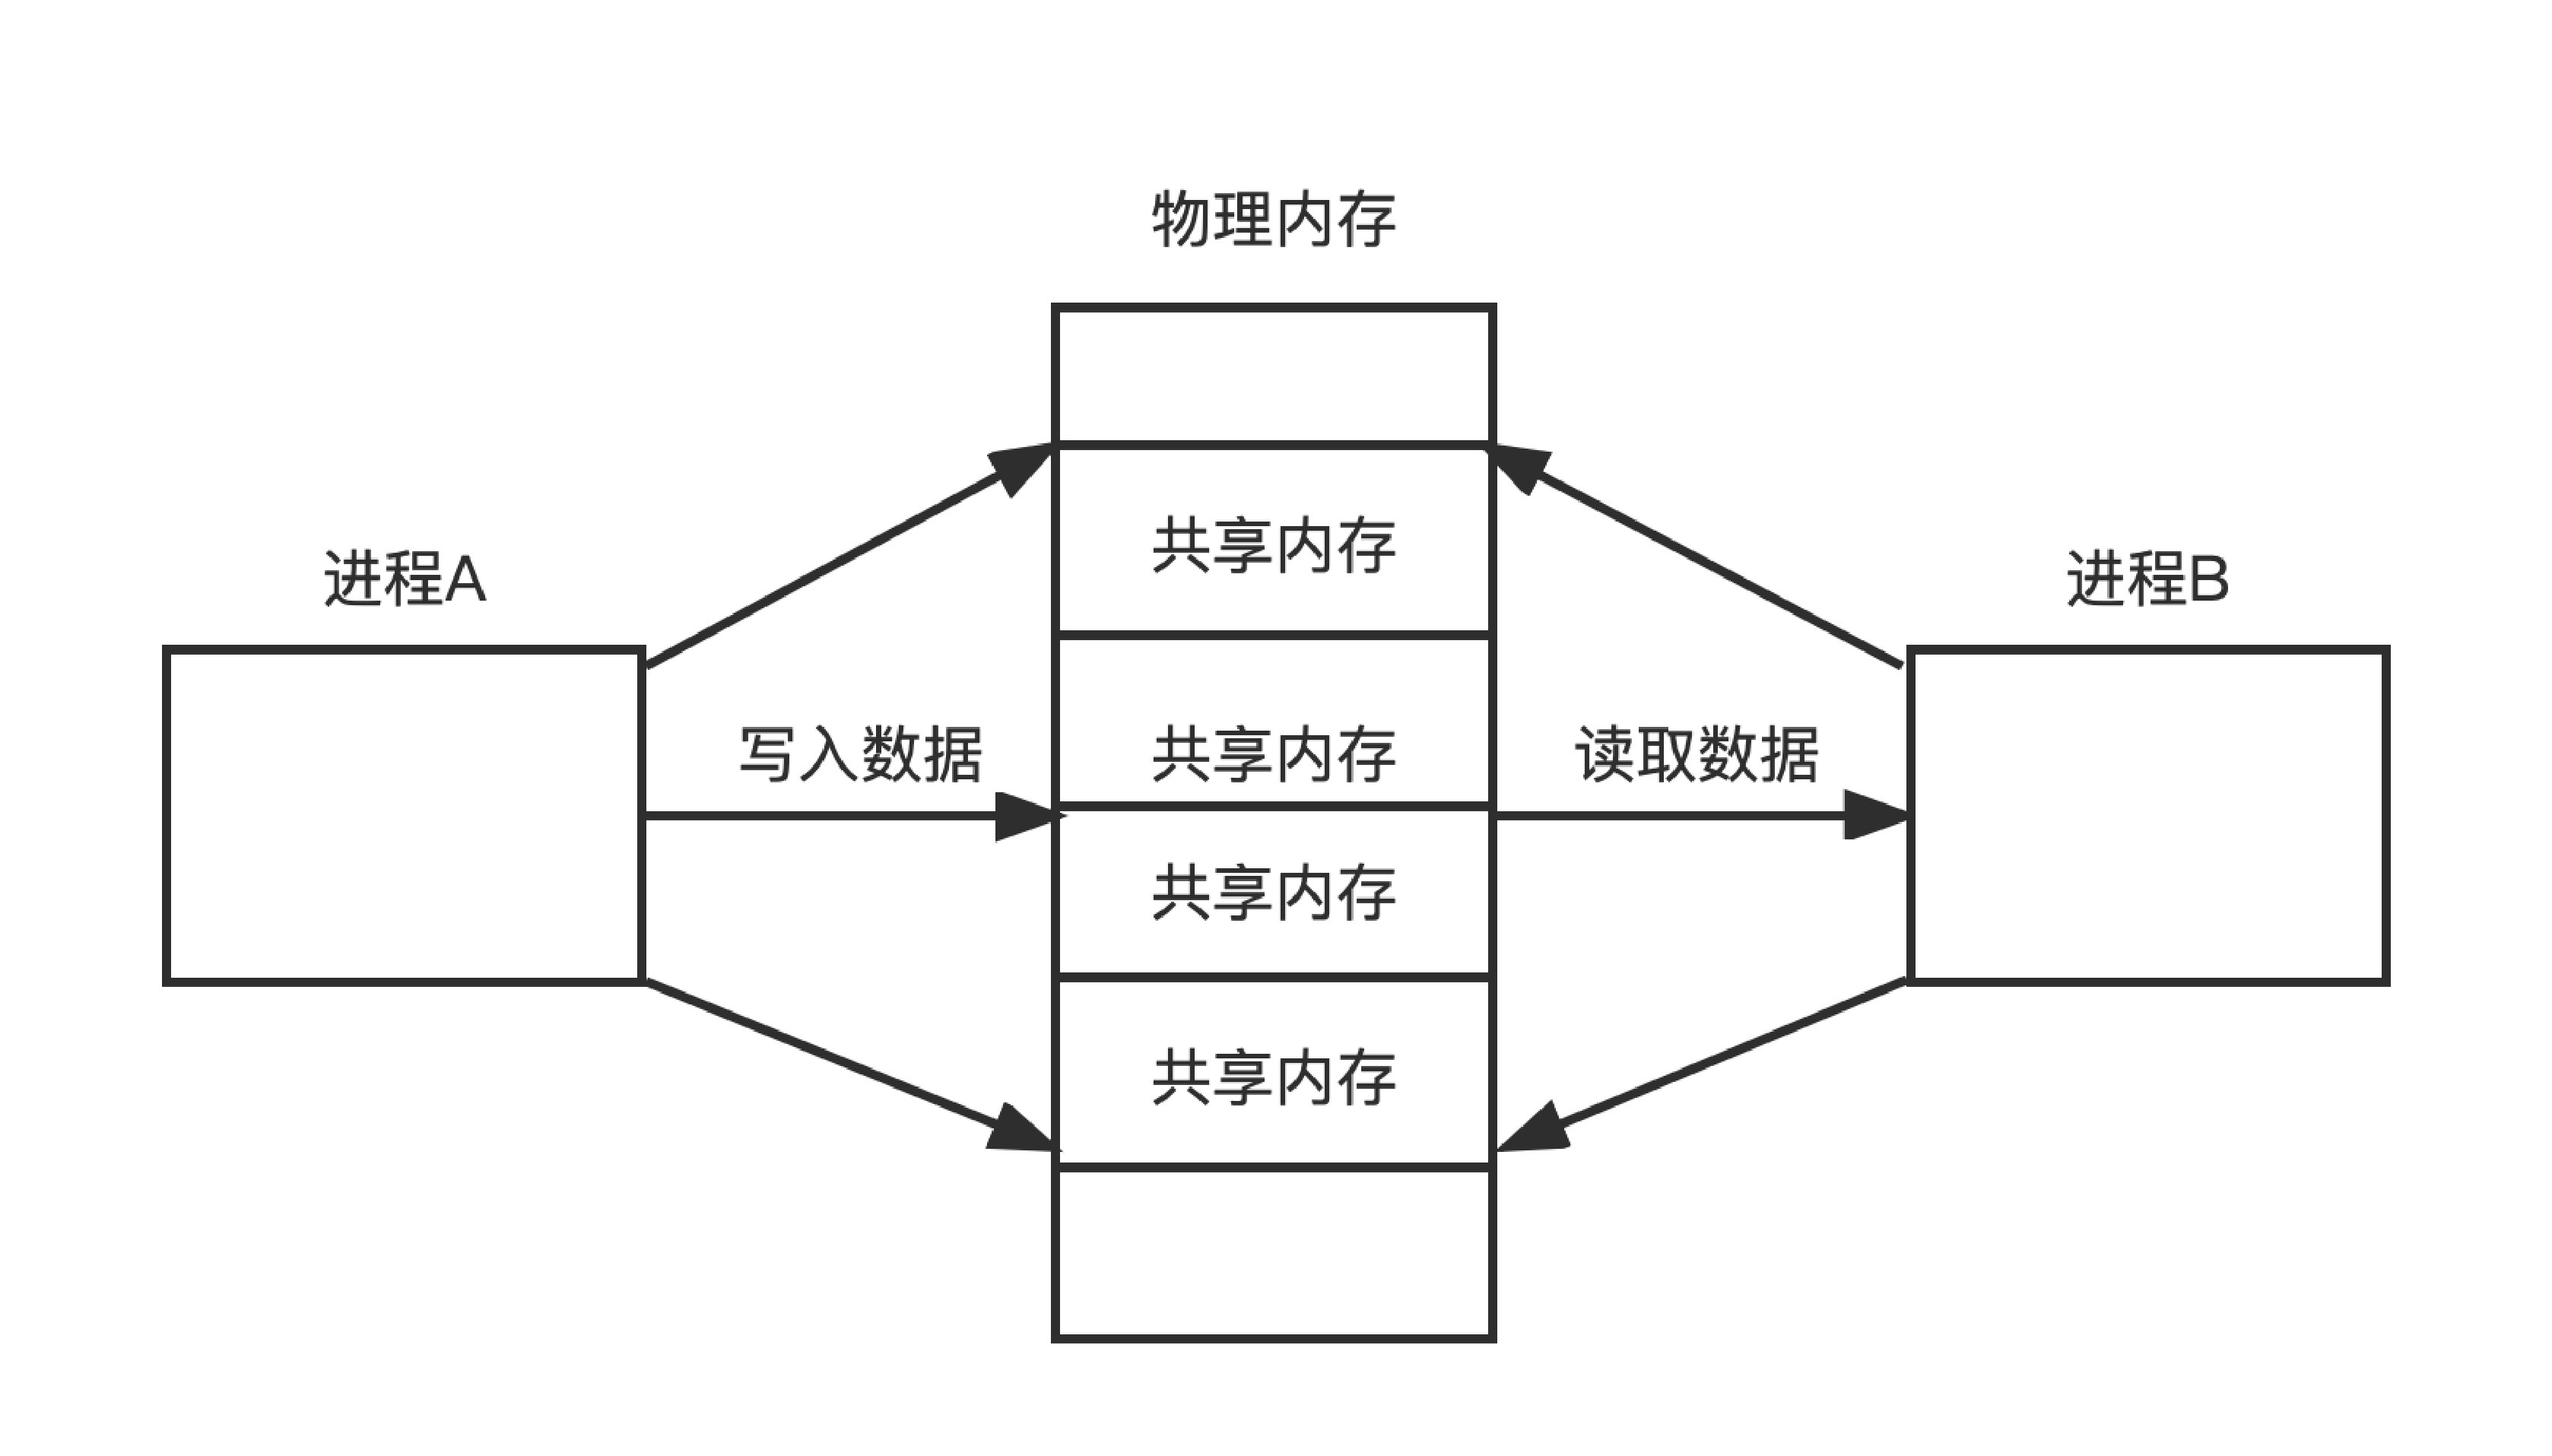
\includegraphics[width=0.65\textwidth]{shared_memory_introduction.pdf}}
  \subfigure[TCP socket]{
    \label{IPC_compare_2}
    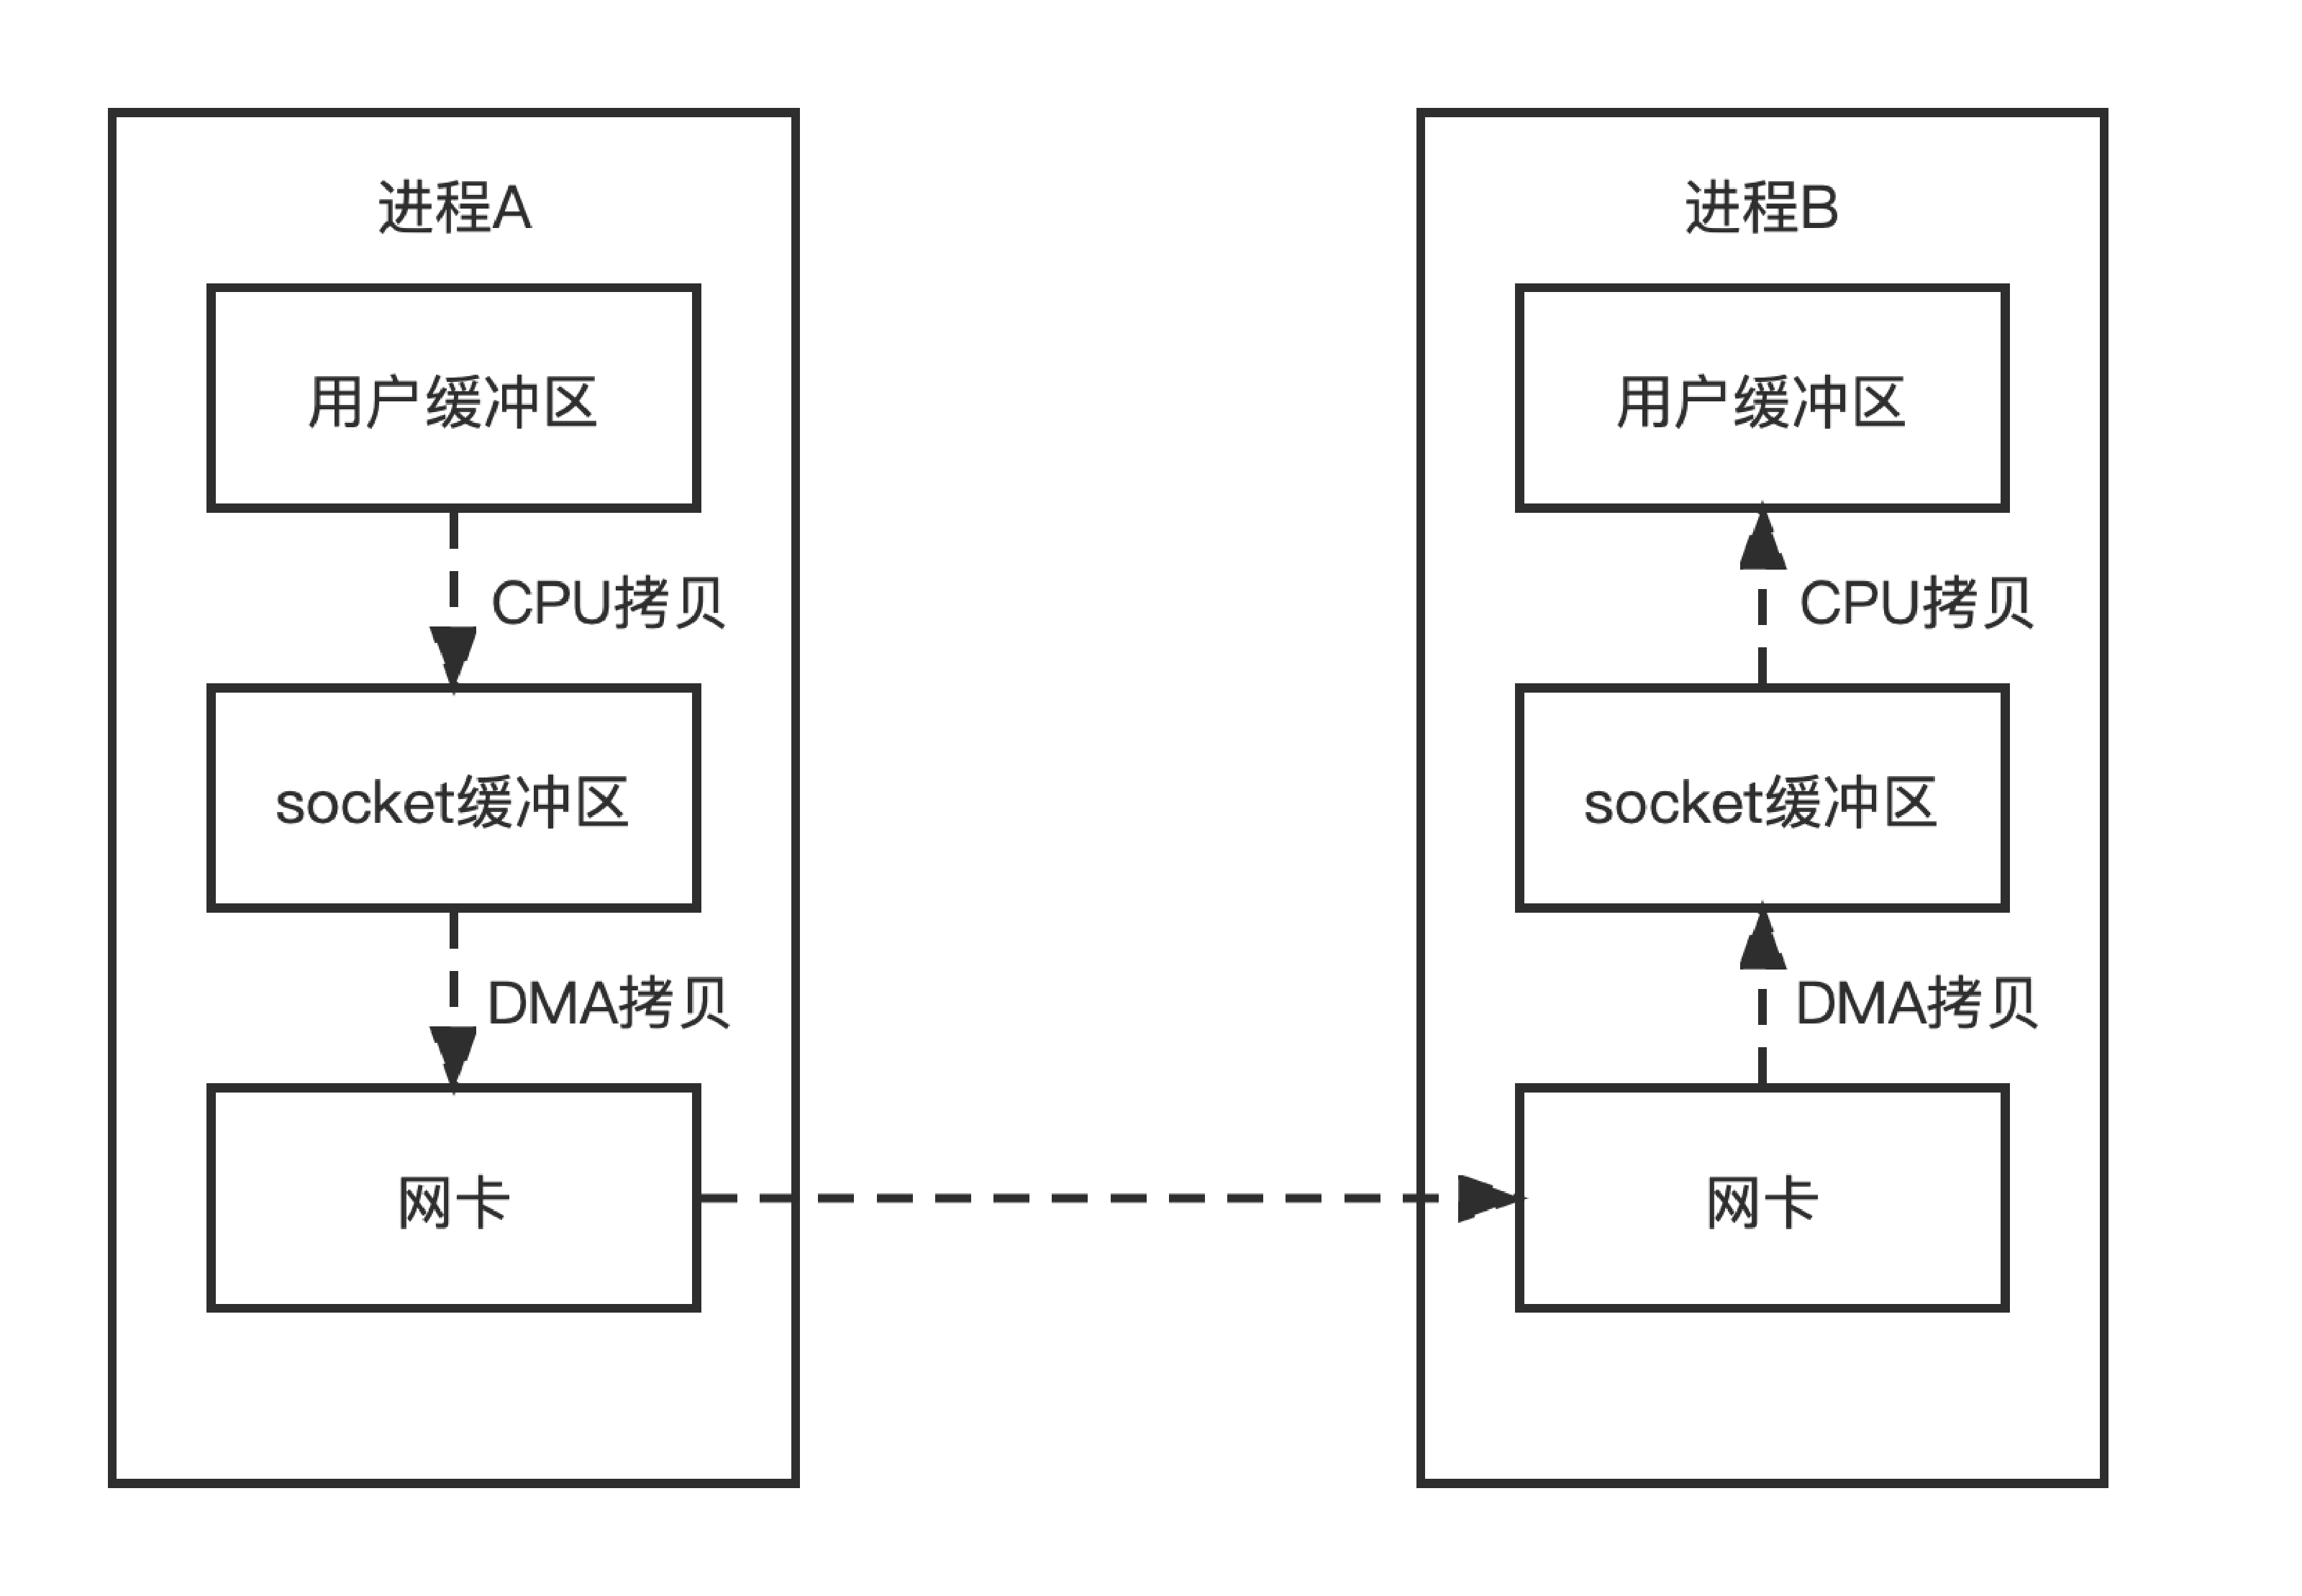
\includegraphics[width=0.6\textwidth]{tcp_socket_introduction.pdf}}
  \caption{共享内存与TCP socket读写过程对比}
  \label{IPC_compare}
\end{figure}
从图\ref{IPC_compare_1}和图\ref{IPC_compare_2}可以看出,使用共享内存读写数据过程中只会发生两次数据拷贝,一次是将数据写入共享内存中
一次是从共享内存中读取数据;而使用TCP socket在读写数据过程中会发生四次数据拷贝。使用进程间通信传输本身就
比较小的数据时,拷贝次数对于系统性能及延迟的影响可以忽略不计,但传输大数据时会明显造成系统通信延迟的上升以及性能
的下降。不仅如此,在本系统内会发生一个发布者向多个订阅者发送消息,这会造成同一份数据被拷贝数十次。
表\ref{data_copy_compare}总结了常见的自动驾驶通信系统使用进程间通信传输一次数据期间发生的拷贝次数。
表\ref{IPC_output_compare}是常用几种进程间通信方式吞吐量性能对比。
\begin{table}[H]
  \centering\small
  \caption{自动驾驶通信系统数据拷贝次数总结\cite{8968462}}
  \label{data_copy_compare}
  \setlength{\tabcolsep}{10mm}{
  \begin{tabular}{ccc}
    \toprule
    进程间通信方法 & 通信系统 & 拷贝次数 \\
    \midrule
    \multirow{3}{*}{Socket} & ROS1 & $1+3\times sub$ \\ & ROS2 & $3+3\times sub$ \\ & LCM\cite{2010LCM} & $1+3\times sub$ \\
    \multirow{2}{*}{共享内存} & Ach\cite{2012Robust} & $1+1\times sub$ \\ & ETHZ-ASL & $1+1\times sub$ \\
    \bottomrule
  \end{tabular}
  }
  \note{注:$sub$代表同一个话题被订阅的次数。}
\end{table}

\begin{table}[H]
  \centering\small
  \caption{不同进程间通信方式吞吐量对比}
  \label{IPC_output_compare}
  \begin{tabular}{ccccc}
    \toprule
    \diagbox{通信方式}{数据量} & 128$\times$1000 & 512$\times$1000 & 2048$\times$1000 & 4096$\times$1000\\
    \midrule
    SHM & 774MB/s & 2072MB/s & 5391MB/s & 7480MB/s \\
    TCP socket & 249MB/s & 760MB/s & 1971MB/s & 2815MB/s \\
    PIPE & 153MB/s  & 515MB/s & 1670MB/s & 2287MB/s \\
    FIFO & 144MB/s & 481MB/s & 1566MB/s & 2343MB/s \\
    \bottomrule
  \end{tabular}
  \note{注:表格中数据量单位为(Byte\ $\times$次数);SHM为共享内存,PIPE为匿名管道,FIFO为命名管道。
  吞吐量测试均未对临界数据进行加锁保护。不同的测试环境数据可能出现不同。}
\end{table}
从表\ref{data_copy_compare}和\ref{IPC_output_compare}可以看出,共享内存的吞吐量相较于其他进程间通信方式在吞吐量和减少消息拷贝方面有明显的优势。
虽然共享内存的优点很多,但也有不可忽视的缺点:
共享内存没有提供数据同步的功能,这代表如果要使用共享内存来进行数据的读写需要使用者自身保证对临界资源的保护。
本文选用共享内存作为进程间通信手段的同时,通过重新设计共享内存数据结构改进了第一章提到的现有共享内存数据结构的缺陷,

\section{自动驾驶操作系统}
自动驾驶系统是典型的多域混合关键系统,对算力、存储容量、操作系统等的要求较高,操作系统对于自动驾驶来说是
最重要的一环\cite{fuyong}。

目前自动驾驶行业存在两种主流的操作系统方案,一种是基于Linux内核的方案,另一种是基于RTOS等嵌入式操作系统的方案。两种方案下
的软件架构如图\ref{ad_os_compare}所示。使用基于Linux内核的方案代表厂商有Waymo、Tesla、NVIDIA、百度等,该方案的优点是Linux具备开放、
应用生态良好和工具链齐全的特点,满足自动驾驶系统快速迭代的需求,但难以满足自动驾驶系统对安全性和实时性的需求。使用基于RTOS等嵌入式
操作系统的代表厂商有大众、戴姆勒、雷诺等,该方案的优点是QNX等嵌入式实时内核安全性和实时性较好,但其应用生态差、对AI软件栈
支持一般。

\begin{figure}[H]
  \centering
  \subfigure[Linux]{
    \label{Fig.sub.1}
    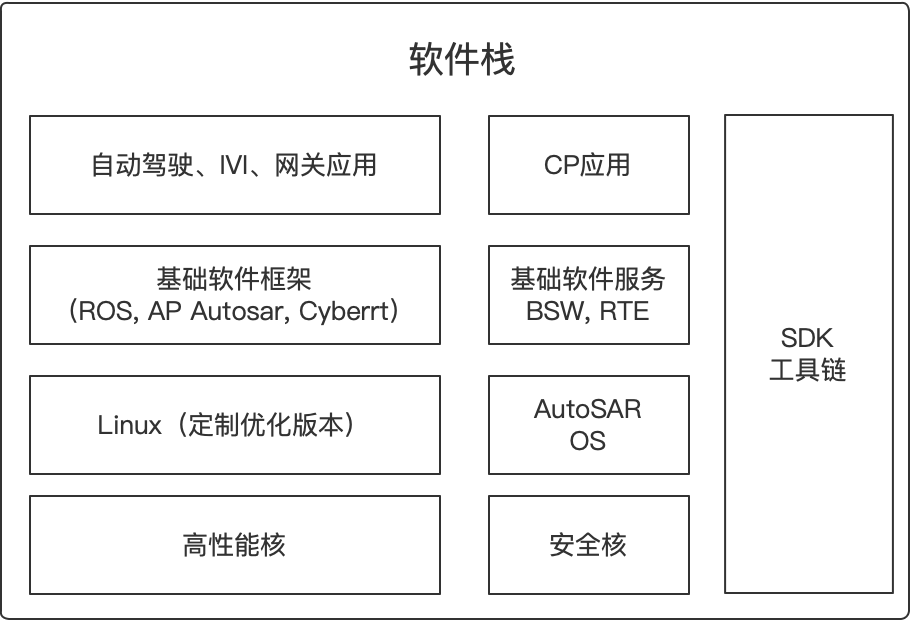
\includegraphics[width=0.7\textwidth]{ADOS_linux.png}}
  \subfigure[嵌入式操作系统]{
    \label{Fig.sub.2}
    \includegraphics[width=0.7\textwidth]{ADOS_RTOS.png}}
  \caption{两种操作系统方案软件架构对比}
  \label{ad_os_compare}
\end{figure}
\section{本章小结}
本章首先介绍了本文系统所使用的ZeroMQ、RPC、序列化技术和共享内存相关的知识,并且阐述本文系统为何要使用这些技术。最后
对自动驾驶操作系统方案进行介绍,比较不同方案各自的优缺点。